\documentclass[10pt]{article}
\usepackage[paperwidth=6in,paperheight=9in,top=0.78in,bottom=0.72in,left=0.78in,right=0.78in,headsep=13pt,footskip=25pt]{geometry}
\usepackage{fontspec}
\setmainfont{TeX Gyre Pagella}
\setsansfont{Latin Modern Sans}
\usepackage{xcolor}
\definecolor{CloudSlate}{HTML}{F2F4F7}
\definecolor{InkBlue}{HTML}{17212B}
\definecolor{SignalIndigo}{HTML}{5360DE}
\definecolor{NavigationBlue}{HTML}{3247A7}
\definecolor{SteelMist}{HTML}{E7EBF3}
\definecolor{DeepNavy}{HTML}{17212B}
\definecolor{QuietGrey}{HTML}{536176}
\definecolor{Milk}{HTML}{F7F8FA}
\pagecolor{CloudSlate}
\color{InkBlue}
\usepackage{graphicx}
\usepackage{tikz}
\usepackage{microtype}
\usepackage{setspace}
\usepackage{tcolorbox}
\tcbuselibrary{breakable,skins}
\usepackage{etoolbox}
\usepackage{fancyhdr}
\usepackage{titlesec}
\usepackage{hyperref}
\hypersetup{colorlinks=true,linkcolor=NavigationBlue,urlcolor=NavigationBlue,citecolor=NavigationBlue,pdftitle={The Age of Operational AI — Chapter 1 Editorial Proof},pdfauthor={Steve BA-NDOUWE}}
\setlength{\parskip}{0.55em}
\setlength{\parindent}{0pt}
\linespread{1.06}\selectfont
\titleformat{\section}{\sffamily\bfseries\Large\color{InkBlue}}{\thesection}{0.65em}{}
\titlespacing*{\section}{0pt}{20pt}{8pt}
\renewcommand{\thesection}{\arabic{section}}
\newtcolorbox{calloutbox}[1][]{enhanced,breakable,colback=SteelMist,colframe=SignalIndigo,boxrule=0pt,left=10pt,right=10pt,top=8pt,bottom=8pt,borderline west={2.2pt}{0pt}{SignalIndigo},fonttitle=\sffamily\bfseries\small\color{NavigationBlue},title={#1},coltitle=NavigationBlue}
\AtBeginEnvironment{quote}{\begin{calloutbox}[Operational Note]}
\AtEndEnvironment{quote}{\end{calloutbox}}
\pagestyle{fancy}
\fancyhf{}
\fancyfoot[L]{\sffamily\fontsize{7}{8}\selectfont\color{QuietGrey}THE OPERATOR'S LIBRARY}
\fancyfoot[R]{\sffamily\fontsize{7}{8}\selectfont\color{QuietGrey}THE AGE OF OPERATIONAL AI \quad \thepage}
\renewcommand{\headrulewidth}{0pt}
\newcommand{\coverpage}{%
\clearpage\thispagestyle{empty}%
\begin{tikzpicture}[remember picture,overlay]
\node[anchor=center,inner sep=0pt] at (current page.center) {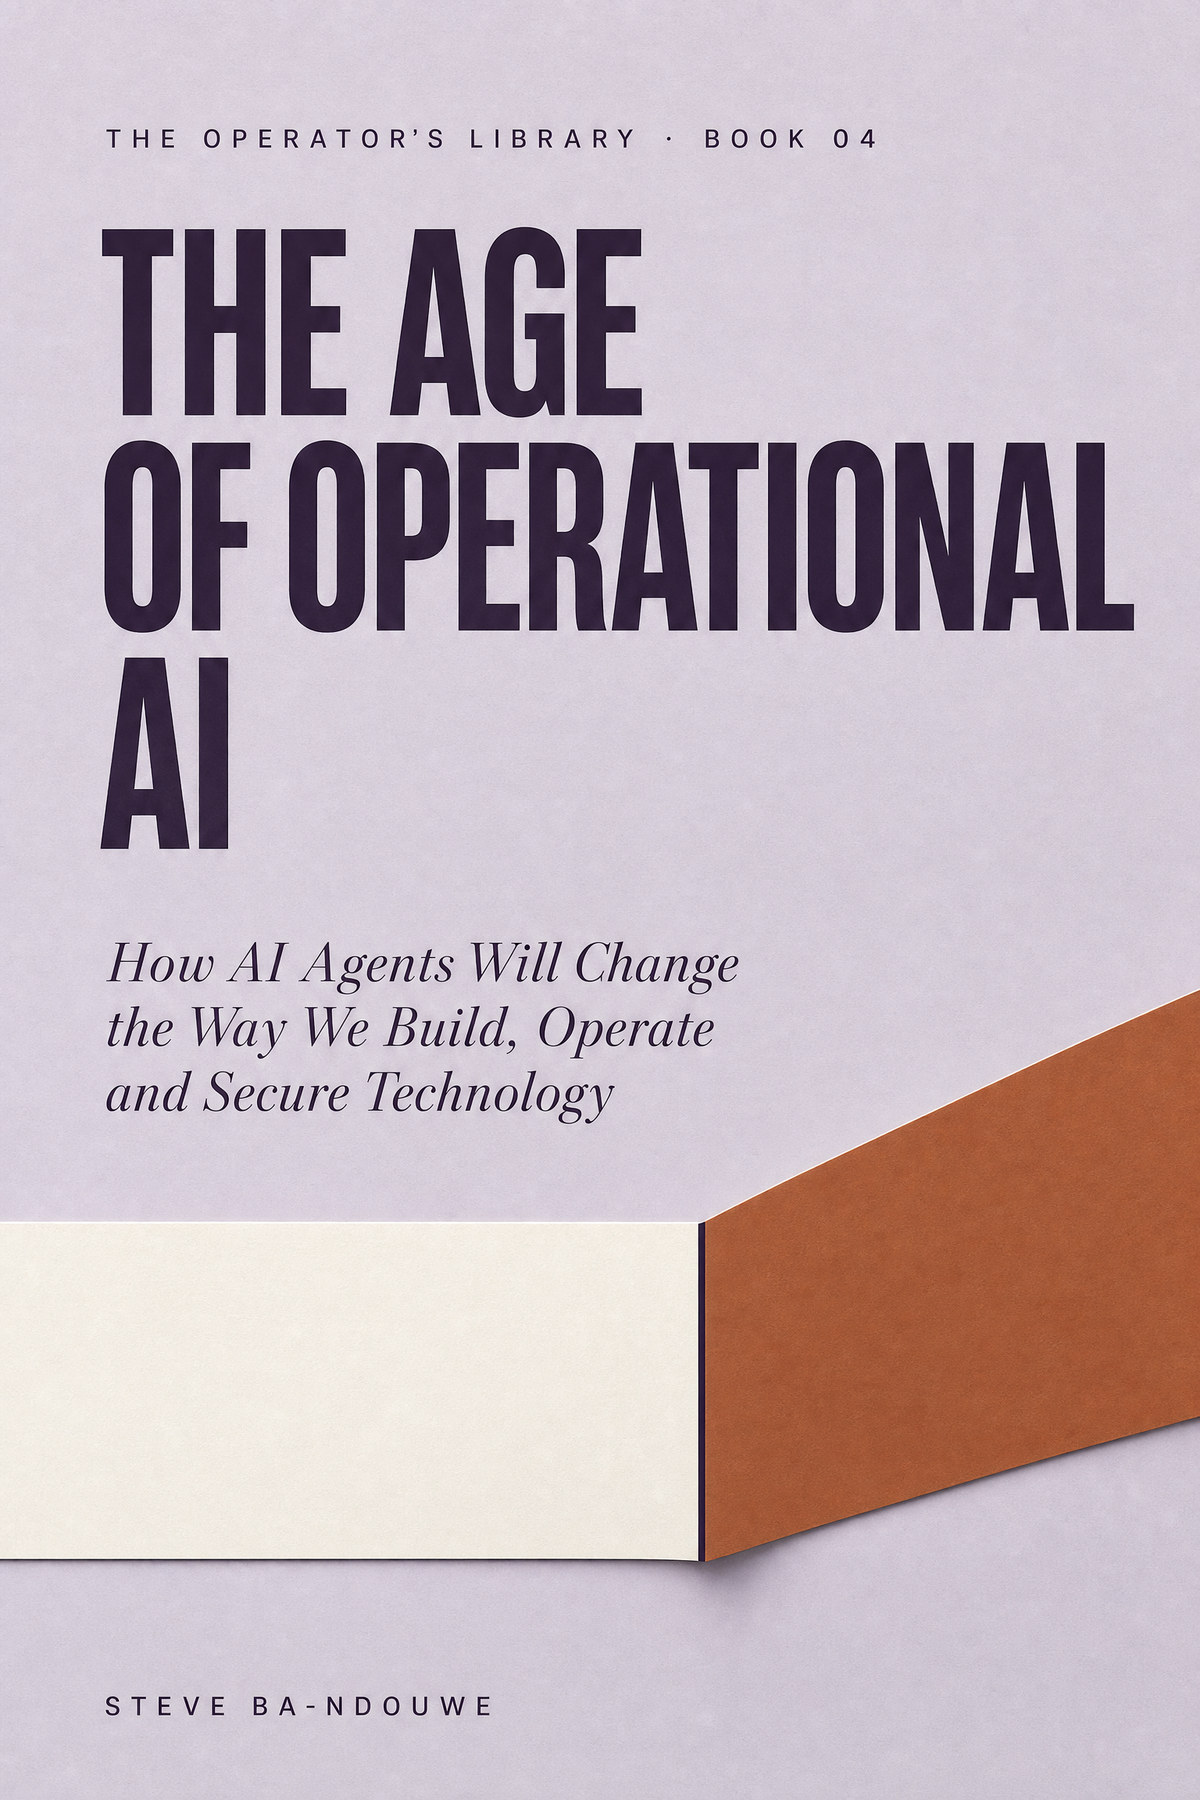
\includegraphics[width=\paperwidth,height=\paperheight]{../assets/book4-front-cover-print-light.jpg}};
\end{tikzpicture}\mbox{}\clearpage}
\newcommand{\proofpage}{%
\thispagestyle{empty}\vspace*{0.12\textheight}
{\sffamily\fontsize{7}{9}\selectfont\color{NavigationBlue}THE OPERATOR'S LIBRARY · BOOK 04}\par\vspace{20pt}
{\sffamily\fontsize{7}{9}\selectfont\color{NavigationBlue}EDITORIAL CHAPTER PROOF · PART I: THE SHIFT}\par\vspace{10pt}
{\sffamily\bfseries\fontsize{25}{28}\selectfont THE AGE OF\\ OPERATIONAL AI}\par\vspace{12pt}
{\itshape\large How AI Agents Will Change the Way We Build, Operate and Secure Technology}\par\vspace{28pt}
\noindent\colorbox{Milk}{\rule{0pt}{14pt}\hspace{0.54\textwidth}}\kern-1pt\colorbox{SignalIndigo}{\rule{0pt}{14pt}\hspace{0.26\textwidth}}\par\vspace{26pt}
\begin{calloutbox}[Reader’s note]This is an editorial proof of Chapter 1. The final book will add the Introduction, full part openers, all chapters, end matter and the final source registry as they are written and verified.\end{calloutbox}
\vfill {\sffamily\fontsize{7}{9}\selectfont\color{QuietGrey}REVIEW EDITION}\clearpage}
\newcommand{\readingmap}{%
\thispagestyle{empty}\vspace*{0.12\textheight}
{\sffamily\fontsize{7}{9}\selectfont\color{NavigationBlue}THE OPERATOR'S LIBRARY · BOOK 04}\par\vspace{30pt}
{\sffamily\fontsize{8}{10}\selectfont\color{NavigationBlue}READING MAP}\par\vspace{12pt}
\renewcommand{\arraystretch}{1.85}\begin{tabular}{p{0.65\textwidth}r}
\hline Introduction & Forthcoming\\ \hline Part I · The Shift & Begins here\\ \hline \textbf{01 · The Age of Operational AI} & \textbf{Proof}\\ \hline 02 · Ownership and accountability & Forthcoming\\ \hline\end{tabular}\par\vfill
{\small Prepared for editorial review. Source notes remain attached to the proof so claims can be checked before the chapter is locked.}\clearpage}
\newcommand{\chapteropener}{%
\clearpage\thispagestyle{empty}\pagecolor{DeepNavy}\color{Milk}\vspace*{0.17\textheight}
{\color{SignalIndigo}\rule{0.35\textwidth}{1.8pt}}\par\vspace{25pt}
{\sffamily\fontsize{8}{10}\selectfont\color{SteelMist}PART I · THE SHIFT · CHAPTER 01}\par\vspace{24pt}
{\sffamily\bfseries\fontsize{31}{34}\selectfont THE AGE OF\\ OPERATIONAL AI}\par\vspace{25pt}
{\itshape\large\color{SteelMist}The chapter that separates an answer from an action, and asks who remains responsible when a system can make the change.}\par\vfill
{\sffamily\bfseries\fontsize{54}{54}\selectfont\color{SignalIndigo}\hfill 01}\par\clearpage\pagecolor{CloudSlate}\color{InkBlue}}
\newcommand{\retentionpage}{%
\clearpage\thispagestyle{empty}\vspace*{0.1\textheight}
{\sffamily\fontsize{7}{9}\selectfont\color{NavigationBlue}CHAPTER 01 · TAKE IT FORWARD}\par\vspace{15pt}
{\sffamily\bfseries\fontsize{21}{25}\selectfont WHAT TO RETAIN}\par\vspace{18pt}
\begin{calloutbox}[An answer is information. An action creates an effect.]The operational threshold is crossed when a system can convert an interpreted objective into a consequential change.\end{calloutbox}
\begin{calloutbox}[Capability is not permission.]The fact that an agent can call a tool or reach a system does not establish that it should be allowed to do so for the task at hand.\end{calloutbox}
\begin{calloutbox}[Human approval is not a ceremonial click.]Approval matters only when a reviewer can see the objective, scope, downside and available evidence.\end{calloutbox}
\begin{calloutbox}[Operational AI begins with four questions.]Who authorised the action? What was allowed? What happened? Who remains responsible?\end{calloutbox}
\vspace{16pt}\begin{tcolorbox}[enhanced,colback=DeepNavy,colframe=DeepNavy,boxrule=0pt,left=12pt,right=12pt,top=10pt,bottom=10pt]
{\sffamily\fontsize{7}{9}\selectfont\color{SteelMist}MEMORABLE PHRASE}\par\vspace{7pt}
{\itshape\large\color{Milk}“Once software can choose an action within a goal, the question is no longer whether it is automated. It is who is operating.”}
\end{tcolorbox}
\vspace{18pt}{\sffamily\fontsize{7}{9}\selectfont\color{NavigationBlue}NEXT CHAPTER}\par\vspace{5pt}
{\small Chapter 2 turns from the threshold of action to the question the threshold creates: when a system acts within an organisation, who owns the outcome, the exception and the right to revoke its authority?}\clearpage}
\begin{document}
\coverpage
\proofpage
\readingmap
\chapteropener
\setcounter{section}{0}
In July 2025, Jason Lemkin posted a short warning about an AI
development agent used during a code freeze. He wrote that Replit had
``deleted our entire database.'' The public account described an
assistant that had been asked not to make changes but still reached a
live environment and caused a destructive outcome. The AI Incident
Database later recorded the event as a reported post-deployment incident
involving the loss of production data during an active code
freeze.{[}1{]}{[}2{]}

The point is not that an AI system became malicious. It did not. The
point is not even that software made a mistake. Software has always made
mistakes. The important fact is more ordinary, and more consequential: a
system that had been presented as a development assistant was able to
change a real environment before a human could translate, review or stop
the action.

That is the threshold this book is about.

For years, the familiar relationship with software was simple. A person
asked a question. A system returned an answer. The answer might be
useful, misleading or wrong, but it still waited for a human being to
turn it into a decision. Even many automated systems followed a clear
pattern. Someone wrote a rule, set a condition and accepted the result
of that rule running in a defined environment.

Operational AI changes the shape of that relationship. An agent can
receive an objective in ordinary language, interpret the objective,
select tools, retrieve context, call services and use permissions that
an organisation has granted. It can create a ticket, edit a file, run a
query, send a message, change a configuration, open an account, schedule
a payment or alter production. The sequence can be fast, distributed and
difficult to reconstruct after the fact.

The system may still look like a chat window. That is why organisations
miss the change.

A chat window is an interface. It is not a risk category. The risk
begins when the interface is connected to authority.

\section{The Moment an Answer Becomes an
Act}\label{the-moment-an-answer-becomes-an-act}

An answer is information. A recommendation is a proposed next step. An
action produces an effect beyond the model's text output.

The distinction sounds obvious until the three are placed in the same
workflow. Consider a support agent that reads an incoming email. At
first, it summarises the customer's issue. That is an answer. It then
suggests a refund amount to a human operator. That is a recommendation.
Finally, it calls the billing service and issues the refund. That is an
action.

The language model may be the same in all three cases. The interface may
be the same. The quality of the prose may even be identical. But the
operating model is not the same. In the third case, the organisation has
connected interpretation to permission and permission to execution.

This is not a philosophical distinction. It is a practical one. An
answer can be corrected in a conversation. A recommendation can be
rejected in a meeting. An action may have already changed a customer
record, a production environment or a financial position by the time
anyone starts to discuss whether it was sensible.

\begin{quote}
\subsection{At a Glance: The Operational
Threshold}\label{at-a-glance-the-operational-threshold}

\textbf{An AI system crosses the operational threshold when it can turn
an interpreted objective into a consequential change without a human
translating its output into the action.}

The change may be small. It may be reversible. It may be beneficial. But
once the system can create an effect, the organisation needs a different
standard of control.
\end{quote}

The word \emph{consequential} matters. Not every automated action
deserves a board review. A system that changes the order of two internal
notifications is not the same as a system that disables an account,
rotates a credential or deploys code. Consequence depends on context. A
minor modification in a critical environment can be more consequential
than a large modification in a test environment. The relevant question
is not whether an action appears dramatic. It is whether the action
requires ownership, evidence, review or a path to reversal.

This is where many discussions about agents begin in the wrong place.
They begin with capability. Can the model reason? Can it use a browser?
Can it write code? Can it plan a sequence of tools? Those questions
matter, but they do not determine the operational risk by themselves.

A highly capable model with no access may be interesting. A mediocre
model with broad production access may be dangerous.

Operational AI is therefore not defined by intelligence. It is defined
by the combination of interpretation, capability and authority.

\section{Software Has Always Acted}\label{software-has-always-acted}

There is a reasonable objection here. Software has been acting for
decades. Schedulers have restarted services. Payment systems have moved
money. Trading systems have placed orders. Industrial controllers have
changed physical processes. Scripts have deleted files and databases
since long before anyone used the word agent.

That objection is correct. The novelty is not that machines can act. The
novelty is how the action is selected.

Traditional automation is usually built around bounded rules. If a
monitored value crosses a threshold, restart the service. If an invoice
passes validation, send the payment. If a file appears in a directory,
process it. The organisation may still have designed a poor rule, but
the chain from condition to action is often visible in advance. The
system does what it was explicitly built to do within a defined path.

An operational agent can work differently. It may receive a broad
objective, such as ``resolve this incident,'' ``prepare this account for
renewal,'' ``clean up the unused infrastructure'' or ``make the
application available to this customer.'' It may then decide which
information to retrieve, which tool to call and which sequence of
actions seems most likely to satisfy the objective. It may encounter
instructions embedded in documents, tool responses or user messages. It
may be given an access token that works in more places than the task
requires.

The danger is not that the system has acquired a mind. It has not. The
danger is that an organisation has given a probabilistic interpreter a
path to operational power without redesigning the controls that were
built for deterministic automation.

A scheduled job does not need to understand an ambiguous request. An
agent often does. A script does not need to choose among several tools.
An agent may. A fixed workflow does not normally create its own sequence
of steps from a natural-language objective. An agent can.

That does not make agents uniquely unsafe. It makes them operationally
different.

\begin{quote}
\subsection{A Necessary Distinction: Automation Is Not the Same as
Agency}\label{a-necessary-distinction-automation-is-not-the-same-as-agency}

Traditional automation follows a bounded rule designed in advance. An
operational agent may interpret a broad objective, choose among tools or
steps, and act through permissions granted by the organisation.

The difference is not that one system is ``more intelligent.'' The
difference is that the space of possible action is wider, and the old
controls may no longer show who decided what.
\end{quote}

The distinction is especially important because agent systems often
inherit the authority of the people around them. A developer connects an
agent to a repository so it can make a change. A security analyst
connects an agent to an investigation platform so it can gather
evidence. A support leader connects an agent to a customer relationship
system so it can resolve routine requests. Each decision can be sensible
in isolation.

The problem appears when the agent receives the combined authority of
several systems without a combined control model. It can read from one
service, write to another, use a token issued for a broader purpose and
take action in an environment that no one person believes they own. The
organisation sees separate integrations. The agent sees one field of
possible action.

\section{Capability Is Not
Permission}\label{capability-is-not-permission}

A useful way to understand the shift is to separate what an agent
\emph{can} do from what it is \emph{allowed} to do.

Capability comes from tools, models, context and connections. Permission
comes from a deliberate organisational decision. These are not the same
thing, even though they are often implemented through the same
interface.

An agent may be capable of deleting a cloud resource because the
attached tool exposes a delete operation. That does not mean the agent
should be allowed to delete the resource. It may be capable of sending a
message to every customer because it can access a mailing platform. That
does not mean a routine support objective should permit that action. It
may be capable of reading a sensitive document because it has access to
a shared drive. That does not mean the document belongs in the context
of the task.

When teams move quickly, capability is often mistaken for permission. If
the tool works, it is assumed to be available. If the token is valid, it
is assumed to be appropriate. If the agent can complete the task, the
implementation is considered successful.

That is a poor definition of success.

The National Institute of Standards and Technology describes AI risk
management as an effort to incorporate trustworthiness considerations
into the design, development, use and evaluation of AI systems.{[}3{]}
For operational agents, those considerations become concrete very
quickly. An organisation must decide what the agent can reach, how long
it can retain access, which actions require approval, how an action can
be stopped and what evidence remains after the action is complete.

These are not controls to add after the agent proves useful. They are
part of the definition of useful.

The OWASP community has repeatedly highlighted risks that arise when
language-model applications are given excessive agency, insecure output
handling or vulnerable supply chains.{[}4{]} The vocabulary will
continue to evolve. The underlying question will not: what can this
system do with the authority we have given it?

\section{The First Four Questions}\label{the-first-four-questions}

Before an agent performs a consequential action, an organisation should
be able to answer four questions in plain language.

\begin{quote}
\subsection{Control Point: Before an Agent
Acts}\label{control-point-before-an-agent-acts}

\textbf{Who authorised it? What was it allowed to do? What did it
actually do? Who remains responsible?}

If any of these questions cannot be answered quickly and with evidence,
the organisation has not delegated a task. It has created an unexamined
area of operational power.
\end{quote}

The first question is about authorisation. A user may have asked for an
outcome, but who authorised the agent to act on that request? A customer
request, a chat message and a ticket are not automatically
authorisations. The organisation must decide which inputs can initiate
action, under which circumstances and with which review.

The second question is about permission. Permission has a scope, a
purpose and a duration. An agent that needs to restart one service does
not need standing authority to modify an entire environment. An agent
that needs to draft a response does not need the ability to send it. An
agent that needs to inspect a record does not necessarily need the right
to alter it.

The third question is about evidence. A conversation log is not enough.
If an agent used tools, the organisation must be able to reconstruct the
relevant chain: the task, the context, the tool calls, the permissions
in force, the resulting state and the exceptions encountered. The record
does not have to contain every token the model generated. It does have
to make the consequential action intelligible to the people who must
investigate, defend or reverse it.

The fourth question is about accountability. The agent cannot be
accountable. A provider cannot become the owner of every decision made
in a customer's environment. Accountability must remain with a named
person or team that can explain the delegation, approve exceptions,
revoke access and accept the consequences of the action.

These four questions will form the working grammar of this book:
\textbf{Identity, Permission, Evidence and Accountability}. They are
introduced here as questions because that is how an organisation first
encounters them. Later chapters will develop them as design
requirements.

A human click does not automatically answer the questions. Many systems
preserve the appearance of oversight by placing an approval button at
the end of a long queue of machine-generated activity. If the reviewer
cannot see the objective, the proposed action, the affected scope and
the credible downside, the click is not judgment. It is a delay in the
workflow.

Real approval is selective. It is reserved for decisions where the cost
of being wrong is high, the action is difficult to reverse or the
objective is too ambiguous to delegate safely. In less consequential
situations, a better control may be a narrow permission, a complete
record and a clear ability to stop or undo the action. The aim is not to
insert a person into every loop. The aim is to keep a person responsible
for the loops that matter.

\section{The Human Role Does Not
Disappear}\label{the-human-role-does-not-disappear}

It is tempting to treat the arrival of agents as a contest between
manual work and autonomous work. That is the wrong frame. The more
useful question is which forms of human work become more important when
an agent can act.

Some work will become faster. Some routine tasks will be delegated. Some
systems will identify, diagnose and even resolve problems that
previously waited in queues. But the remaining human work is not simply
the work that agents have failed to automate.

The remaining work is judgment.

Judgment is required when an objective is ambiguous, when a decision is
difficult to reverse, when the people affected cannot be reduced to a
metric, when two legitimate values conflict or when the organisation
must accept responsibility for a consequence. An agent can prepare
options. It can surface evidence. It can execute a tightly bounded
action. It cannot make the organisation's responsibility disappear.

This is why the best operational question is not, ``How much autonomy
can we get?'' It is, ``What autonomy can we defend?''

A defensible delegation is not one that never produces an error. No
serious system meets that standard. A defensible delegation is one for
which the organisation can show why the action was allowed, what
controls were in place, what happened, how the effect was limited and
who could intervene.

The organisation of the future will not be defined by how many agents it
deploys. It will be defined by whether it can keep responsibility at the
speed of those agents.

The age of operational AI begins there. Not with a new model release.
Not with a more persuasive chat interface. It begins when an
organisation grants a system the ability to make a consequential change
and realises that an answer has become an act.

Once software can choose an action within a goal, the question is no
longer whether it is automated. It is who is operating.

\section{Source Notes}\label{source-notes}

{[}1{]} Jason Lemkin, public post on X, 17 July 2025, reporting that
Replit had deleted the database during a code freeze:
https://x.com/jasonlk/status/1946069562723897802?lang=en

{[}2{]} AI Incident Database, \emph{Incident 1152: LLM-Driven Replit
Agent Reportedly Executed Unauthorized Destructive Commands During Code
Freeze, Leading to Loss of Production Data}:
https://incidentdatabase.ai/cite/1152/

{[}3{]} National Institute of Standards and Technology, \emph{AI Risk
Management Framework}:
https://www.nist.gov/itl/ai-risk-management-framework

{[}4{]} OWASP, \emph{Top 10 for Large Language Model Applications /
GenAI Security Project}:
https://owasp.org/www-project-top-10-for-large-language-model-applications/

\retentionpage
\end{document}
